%Minimierung leer Thread
\subsection{Minimierung leer laufende Thread}

In CUDA bearbeitet jeder Multiprozessor gleichzeitig mit 32 Threads \cite{cudapg}, die allen zum selben Block gehören. Bei der Sparematrix-Multiplikation sind viele Threads am leerlaufen. Um die Leerlaufenden Threads zu minimieren, müssen mehrere Punktprodukte in einem Block bearbeitet werden. Dazu verwendet man 2 dimensionierte Blocksizes. Die Definition und Anwendung von 2-D Blocksize findet man in der Referenz\cite{cudapg} und \cite{cudbp}. 

% \begin{figure}[htbp]
	% 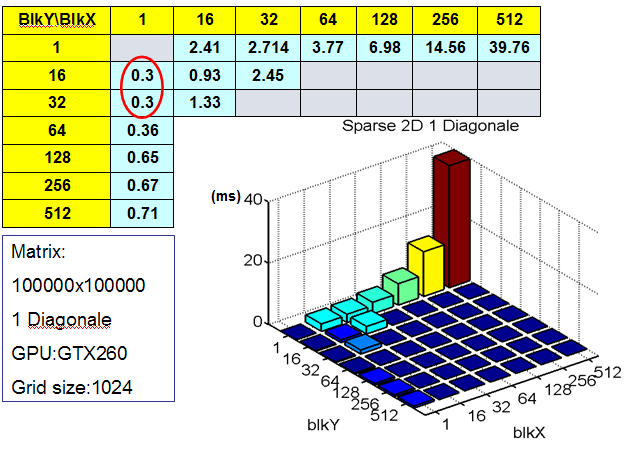
\includegraphics[width=1.7in]{../xby/pic//einDiagonal}
	% \caption{Multipliktion Ein-Diagonalematrize mal Vektor. BlockY: Anzahl der Y-Dimension von Block; BlockX: Anzahl der X-Dimension von Block}
	% 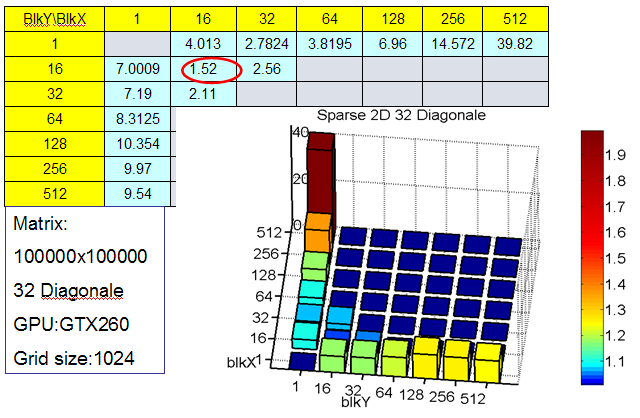
\includegraphics[width=1.7in]{../xby/pic//moreDiagonal}
	% \caption{Multipliktion 32-Diagonalematrize mal Vektor. BlockY: Anzahl der Y-Dimension von Block; BlockX: Anzahl der X-Dimension von Block.}
% \end{figure}